\begin{mainquestion}{superposition}{Superposition}
Consider this circuit that you've solved in a previous assignment:

\begin{center}
    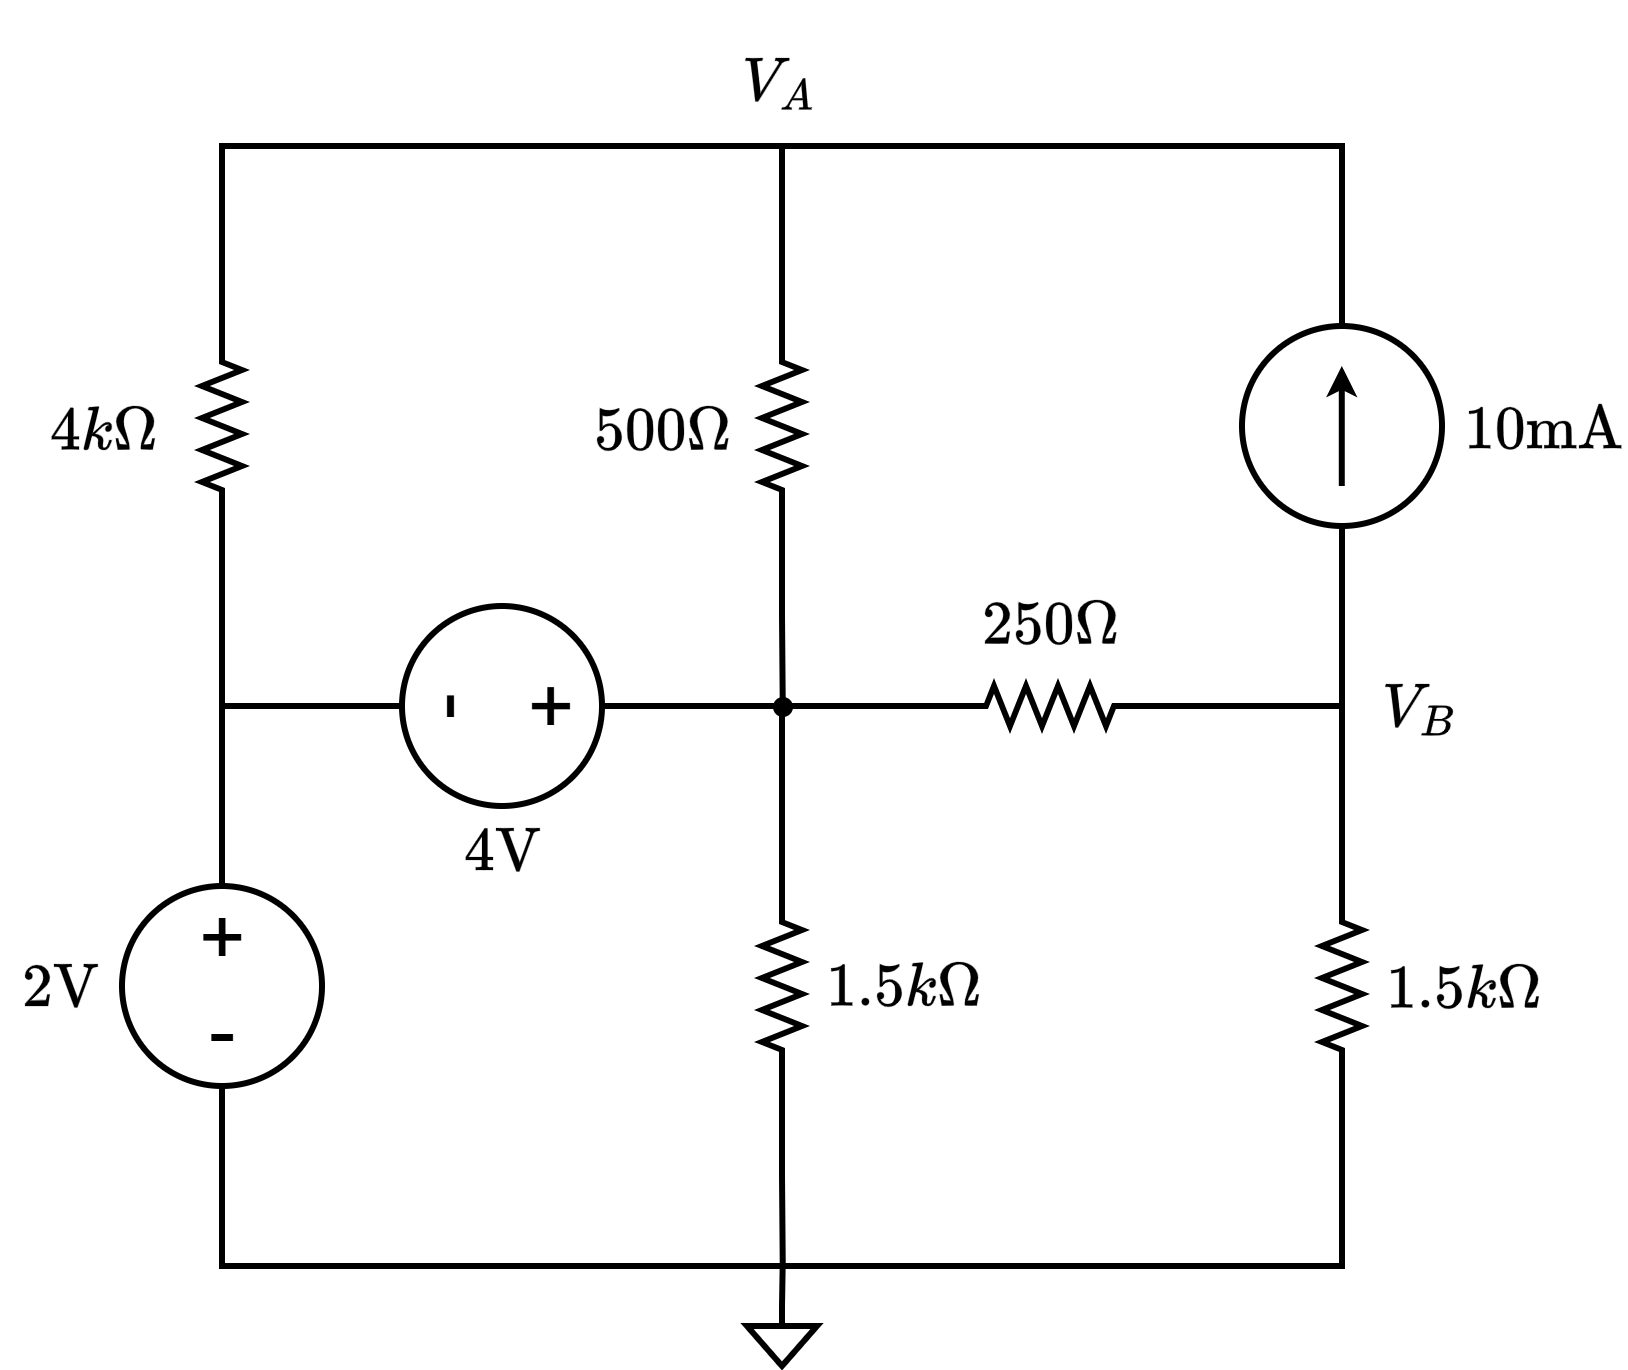
\includegraphics[width=0.8\textwidth]{schematic.png}
\end{center}

\begin{partquestion}{calculatevab}{Use superposition to find $V_A$ and $V_B$.}
\begin{answer}
Superposition tells us that we can consider the effect of each independent source individually. We can do this by disabling all but one of the independent sources (open current sources, short voltage sources) and solving for the voltages at $V_A$ and $V_B$. Then we can add up the contributions to each and we should get the final values of $V_A$ and $V_B$, respectively.
\bigskip

\textbf{2V source only:} open the 10 mA source and short the 4 V source. The circuit becomes:
\begin{center}
    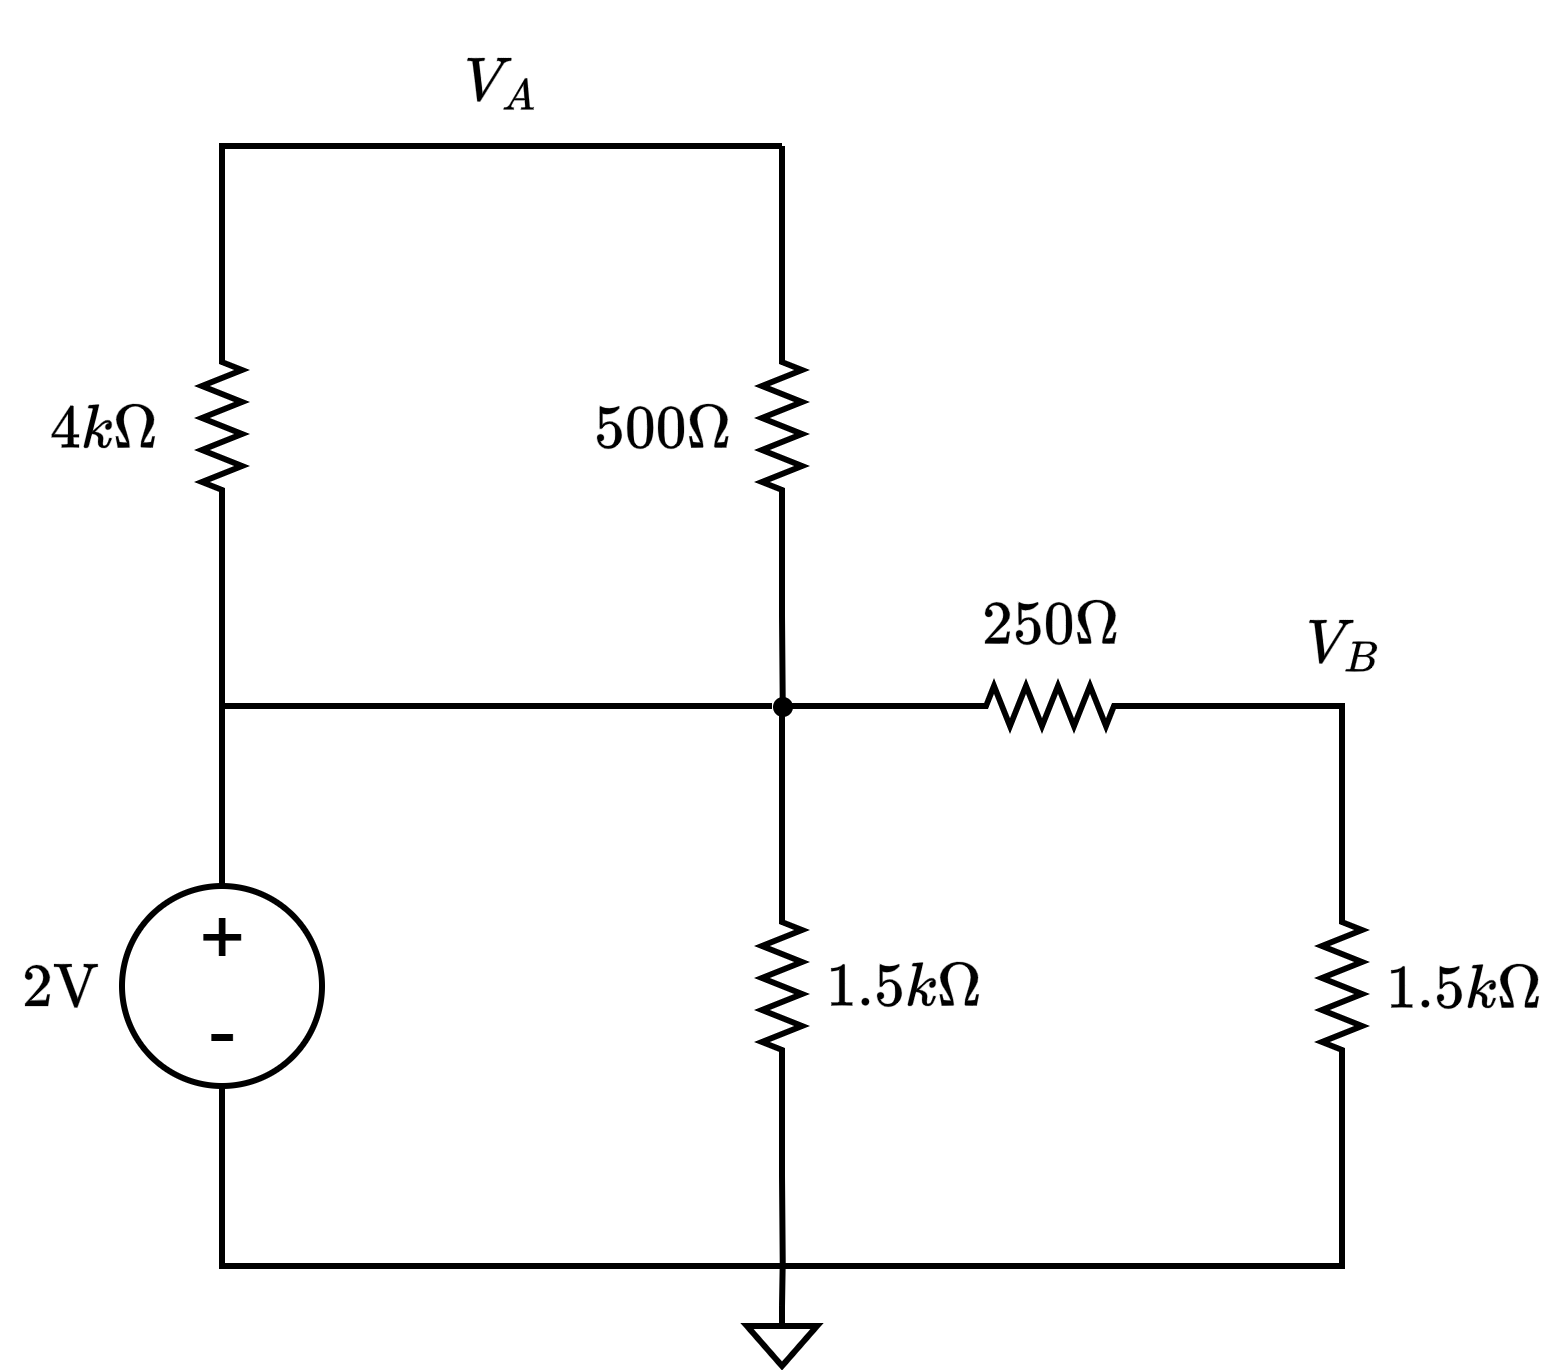
\includegraphics[width=0.6\textwidth]{super_2v.png}
\end{center}

The circuit is now just a resistor network with a single independent source. We see right away that $V_B$ is the output of a voltage divider:
\[
V_B = 2\frac{1500}{1500 +250} = \frac{12}{7}\unit{\volt}
\]
$V_A$ is stranded at the top of the circuit. KVL tells us that the drop across the \qty{4}{\kilo\ohm} resistor and the \qty{500}{\ohm} must add up to zero, but parallel elements must have the same voltage:
\[
V_{\qty{4}{\kilo\ohm}} + V_{\qty{500}{\ohm}} = 0 \hspace{1cm} V_{\qty{4}{\kilo\ohm}} = V_{\qty{500}{\ohm}}
\]

The only solution is if $V_{\qty{4}{\kilo\ohm}}$ and $V_{\qty{500}{\ohm}}$ are both \qty{0}{\volt}! This implies that $V_A$ is the same voltage as the voltage source, so:
\[V_A = \qty{2}{\volt}\]
\bigskip

\textbf{4 V source only:} open the 10 mA source and short the 2 V source. The circuit becomes:
\begin{center}
    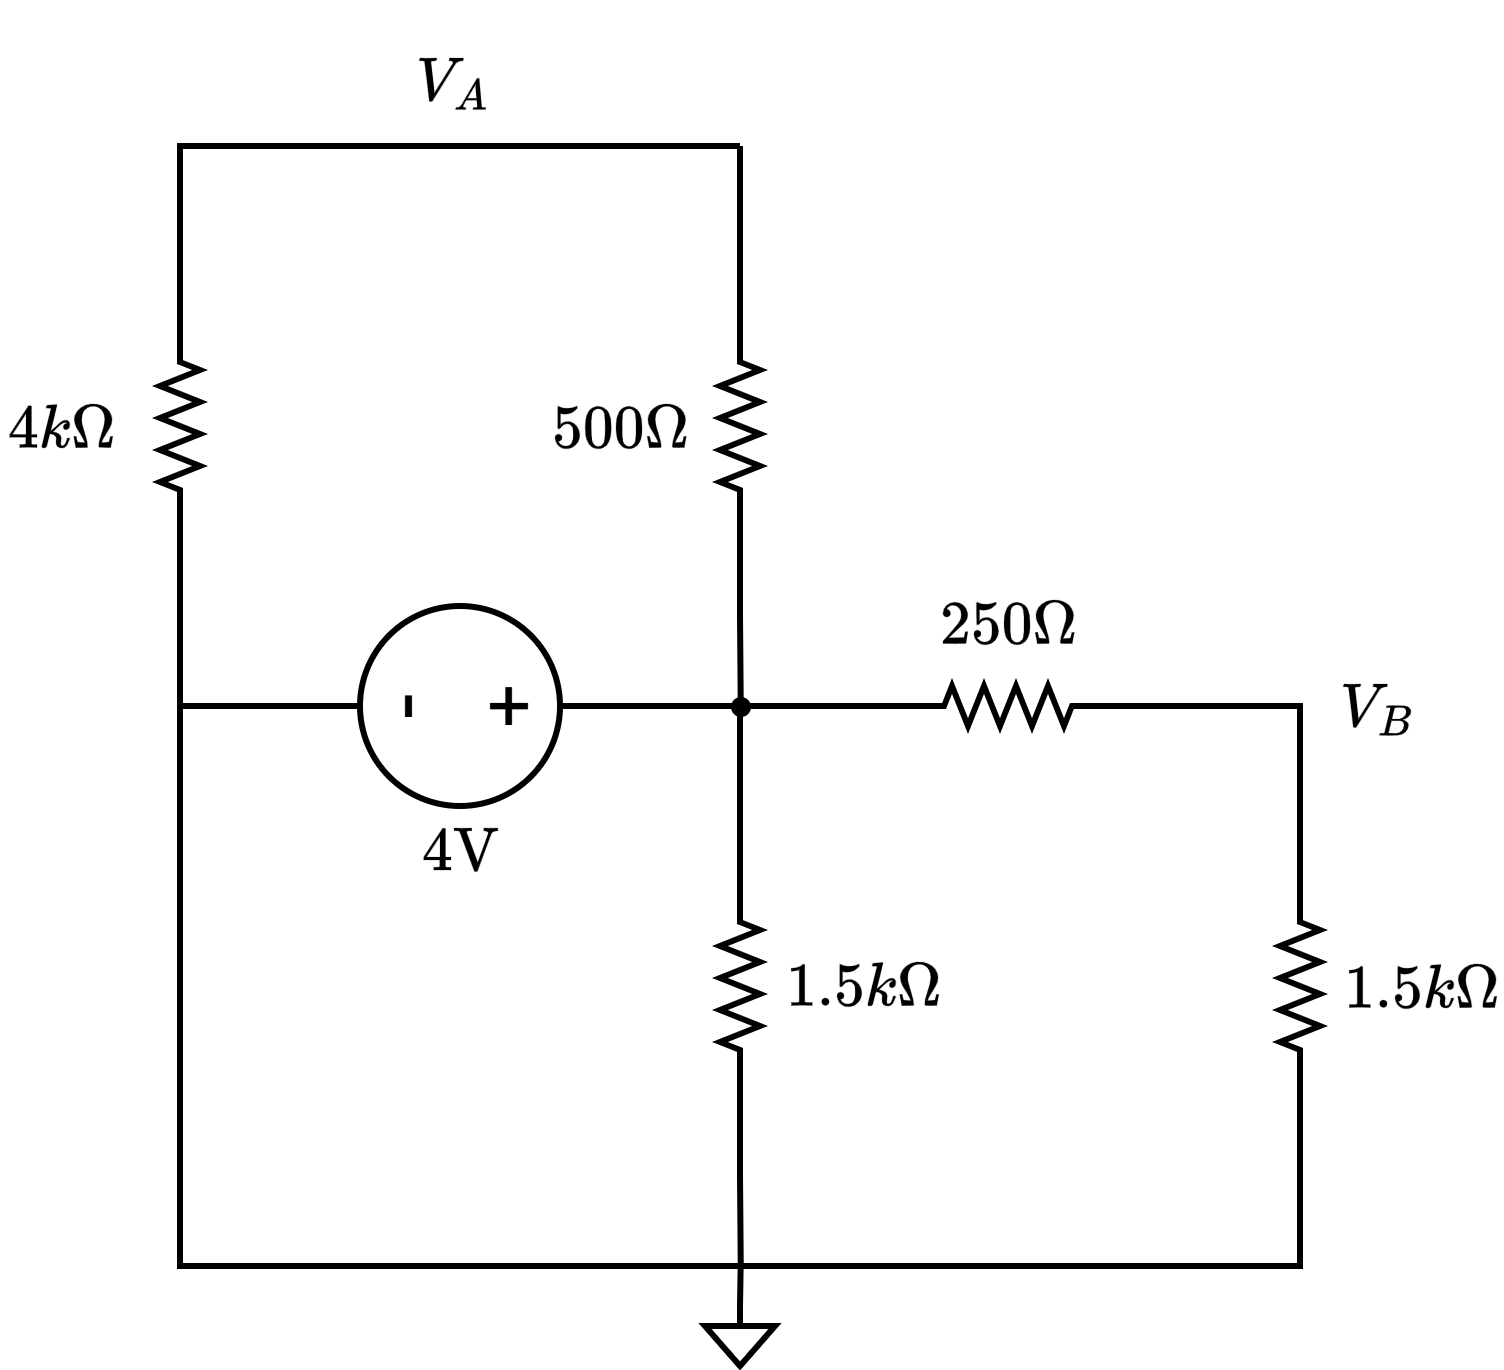
\includegraphics[width=3in]{super_4v.png}
\end{center}

This is very similar to before, except now both $V_A$ and $V_B$ are voltage dividers:
\[
V_A = 4\frac{4000}{4000 +500} = \frac{32}{9}\unit{\volt}
\]

\[
V_B = 4\frac{1500}{1500 +250} = \frac{24}{7}\unit{\volt}
\]
\bigskip

\textbf{10 mA source only:} short both voltage sources. The circuit becomes:
\begin{center}
    \includegraphics[width=3in]{super_10mA.png}
\end{center}

Let's take a second to figure out what we are looking at. The current from our 10mA source will pass through the \qty{4}{\kilo\ohm} resistor and the \qty{500}{\ohm} resistor in parallel before reaching ground. Then the current will pass through the \qty{1.5}{\kilo\ohm} resistor and the \qty{250}{\ohm} resistor in parallel on its way back to the current source. The other \qty{1.5}{\kilo\ohm} is shorted so the current won't bother to flow through it.

The voltages $V_A$ and $V_B$ will be the voltage drops across the effective parallel resistor pairs:

\[V_A = 10 \frac{0.5 \cdot 4}{4 + 0.5} = \frac{40}{9}\unit{\volt}\]
\[V_B = -10 \frac{0.25 \cdot 1.5}{1.5 + 0.25} = -\frac{15}{7}\unit{\volt}\]
Note $V_B$ is negative thanks to our passive sign convention.
\bigskip

Now we can sum our results to find the final values:
\[
V_A = 2 + \frac{32}{9} + \frac{40}{9} = \frac{90}{9} = \qty{10}{\volt}
\]
\[
V_B = \frac{12}{7} + \frac{24}{7} - \frac{15}{7} = \frac{21}{7} = \qty{3}{\volt}
\]
\end{answer}
\end{partquestion}

\begin{partquestion}{compare}{Does your result in part (\cref{prob:superposition:calculatevab}) match your solution from HW2 Problem 1? Which method do you prefer and why?}

\begin{answer}
    Our solution to HW2 Problem 1 found that the voltage across $R_5$ (rightmost \qty{1.5}{\kilo\ohm}) was \qty{3}{\volt} and the voltage across $R_1$ (upper right \qty{4}{\kilo\ohm}) was \qty{8}{\volt}. Given we assign the bottom node to be ground as shown, that would imply $V_A = 2 + 8 = \qty{10}{\volt}$ and $V_B = \qty{3}{\volt}$, a perfect match!
    In this case superposition made our job easier by removing the need to solve any systems of equations.
\end{answer}
\end{partquestion}

\end{mainquestion}
